\subsection{Wichtige Berechnungen}\label{sec:berechnungen}
Mit der Benutzung und der Anwendung der Formel für den schrägen Wurf, konnten die Geschwindigkeit und die notwendige Energie berechnet werden, 
die der Ball braucht um bis zum Korb zu fliegen. Die Berechnungen ergaben, dass die Bälle idealerweise in einer Höhe von ca. 40 cm und unter einem Winkel von ca. 50° abgeworfen werden. Für die Berechnungen wurde ein Rad mit ein Durchmesser von 15 cm benutzt. \\

\begin{figure}[h!]
	\begin{subfigure}{.5\textwidth}
		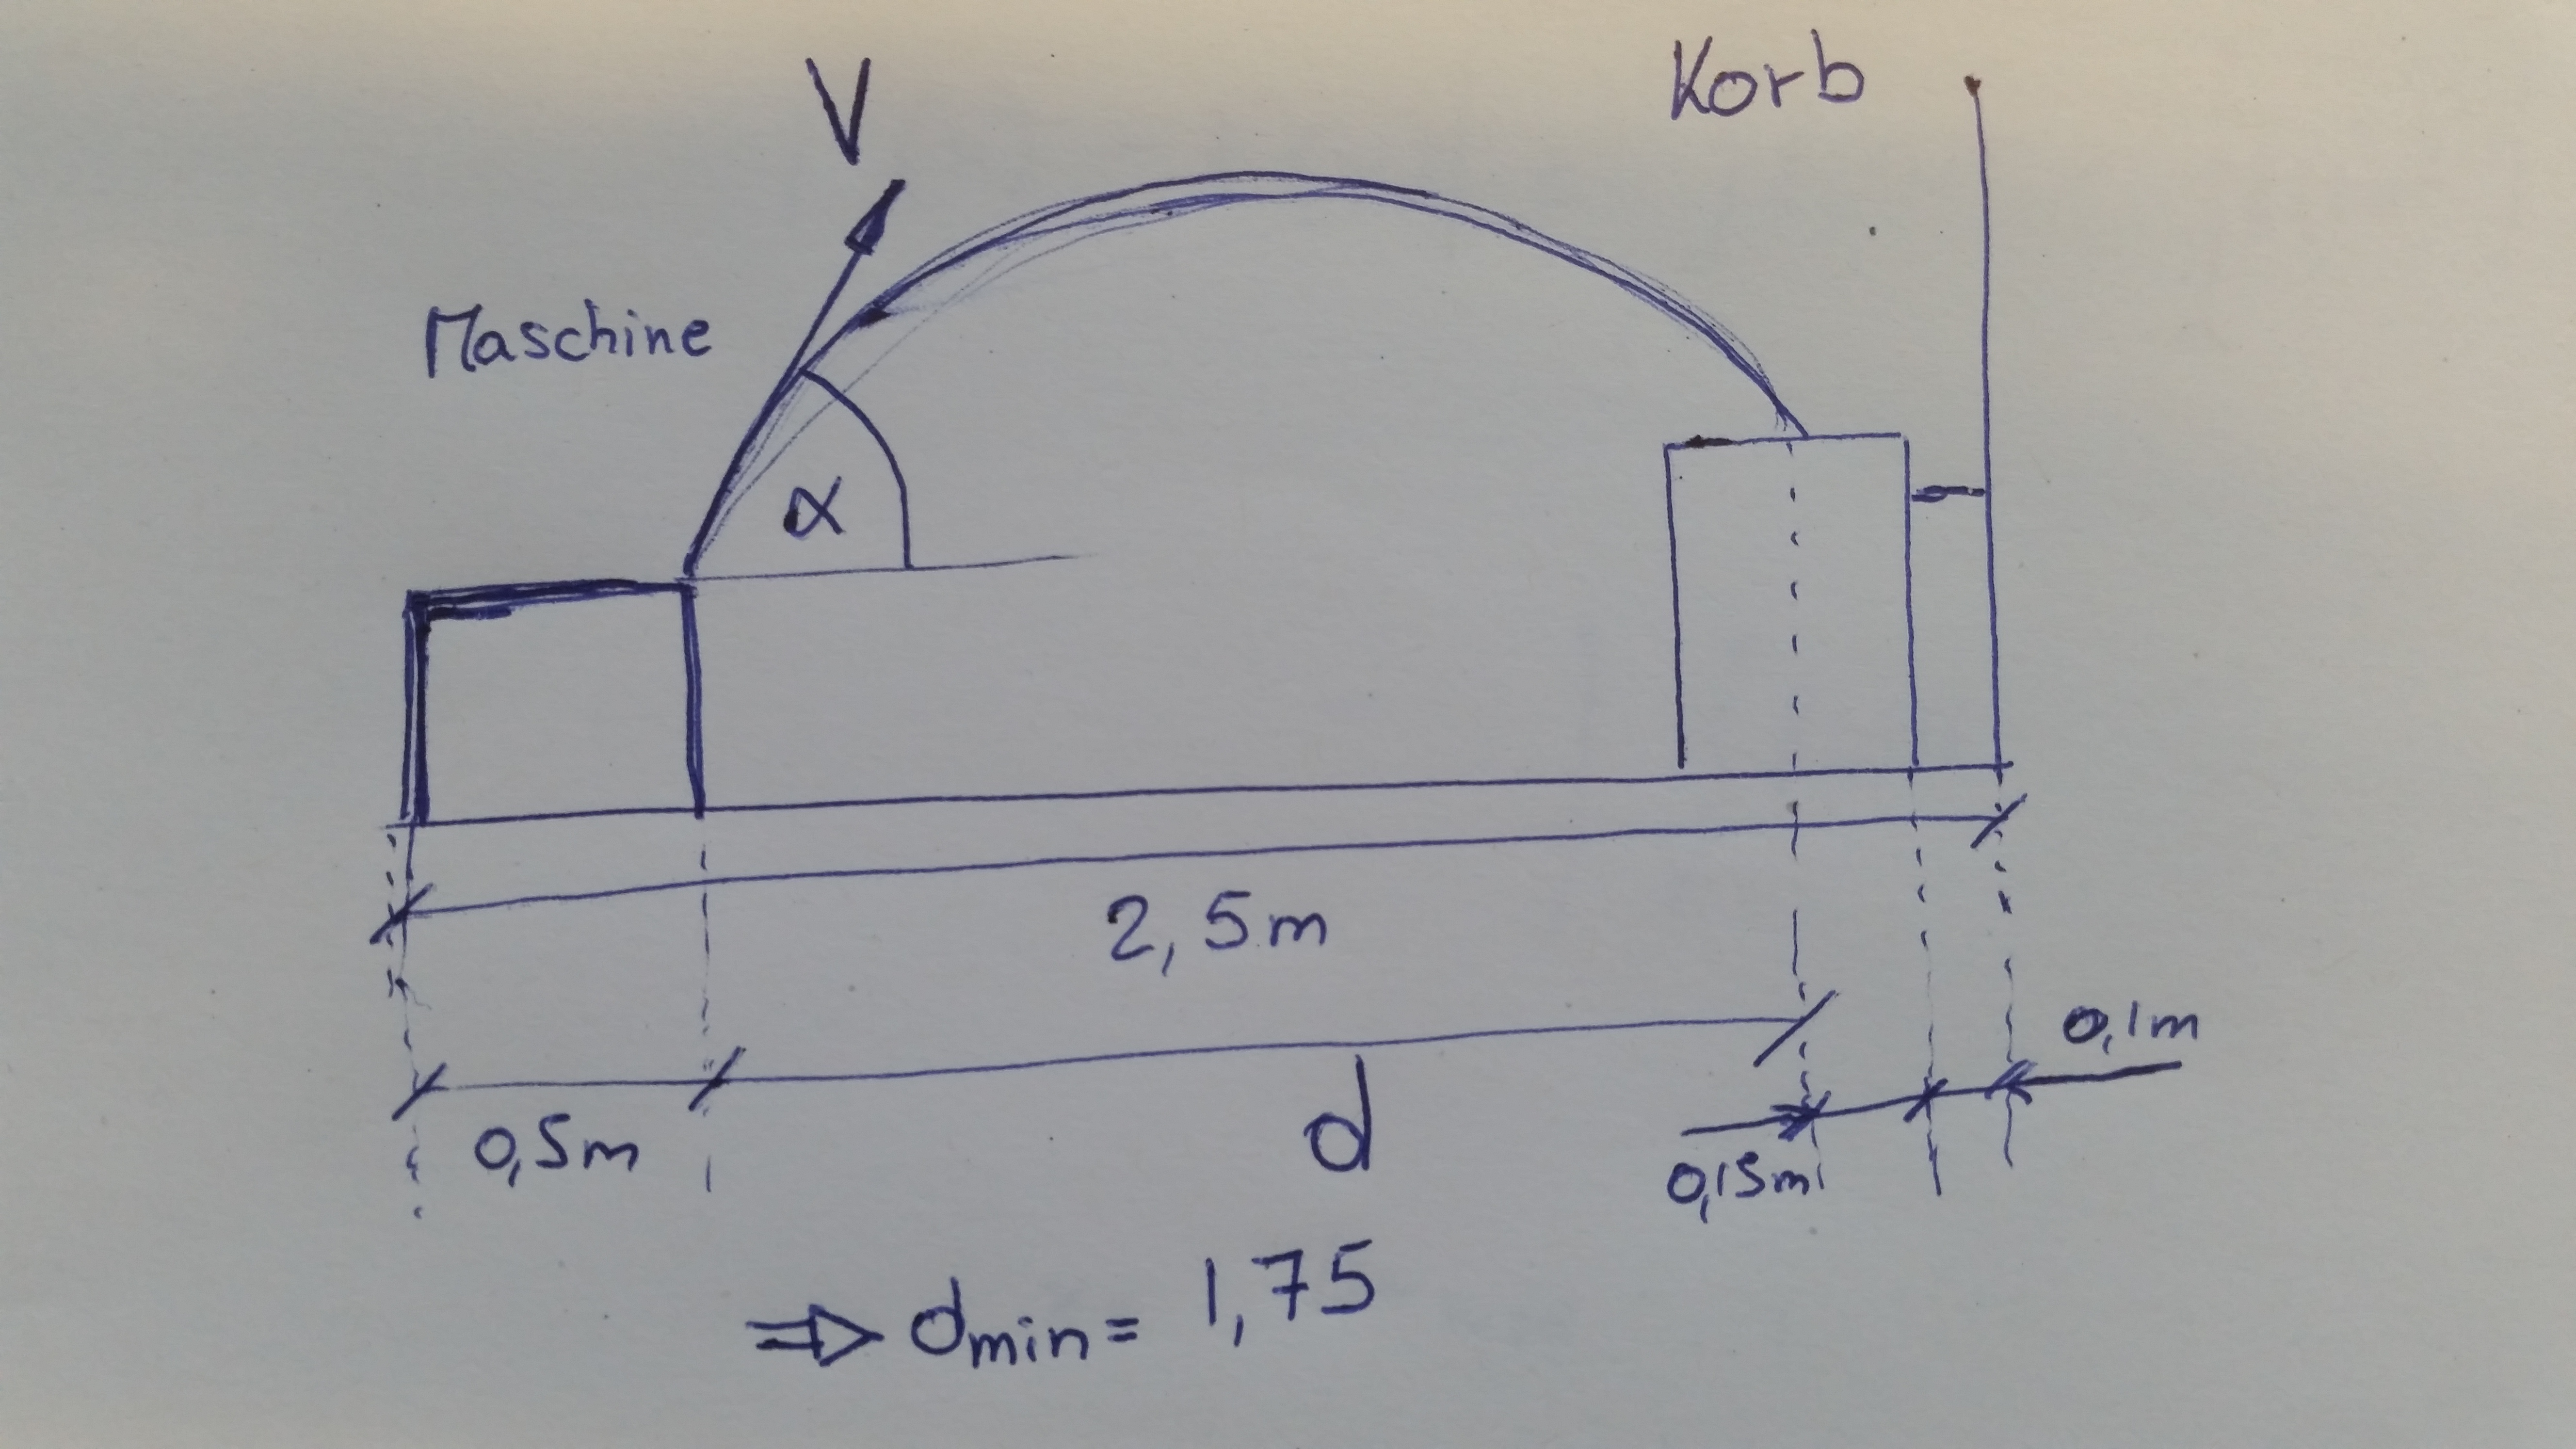
\includegraphics[width=1\textwidth]{../../fig/Skizze_Berechnung_1.jpg}
		\caption{Schrägen Wurf von der Seite}
		\label{fig:Berechnungen von die Geschwindigkeit}
	\end{subfigure} %
	\begin{subfigure}{.5\textwidth}
		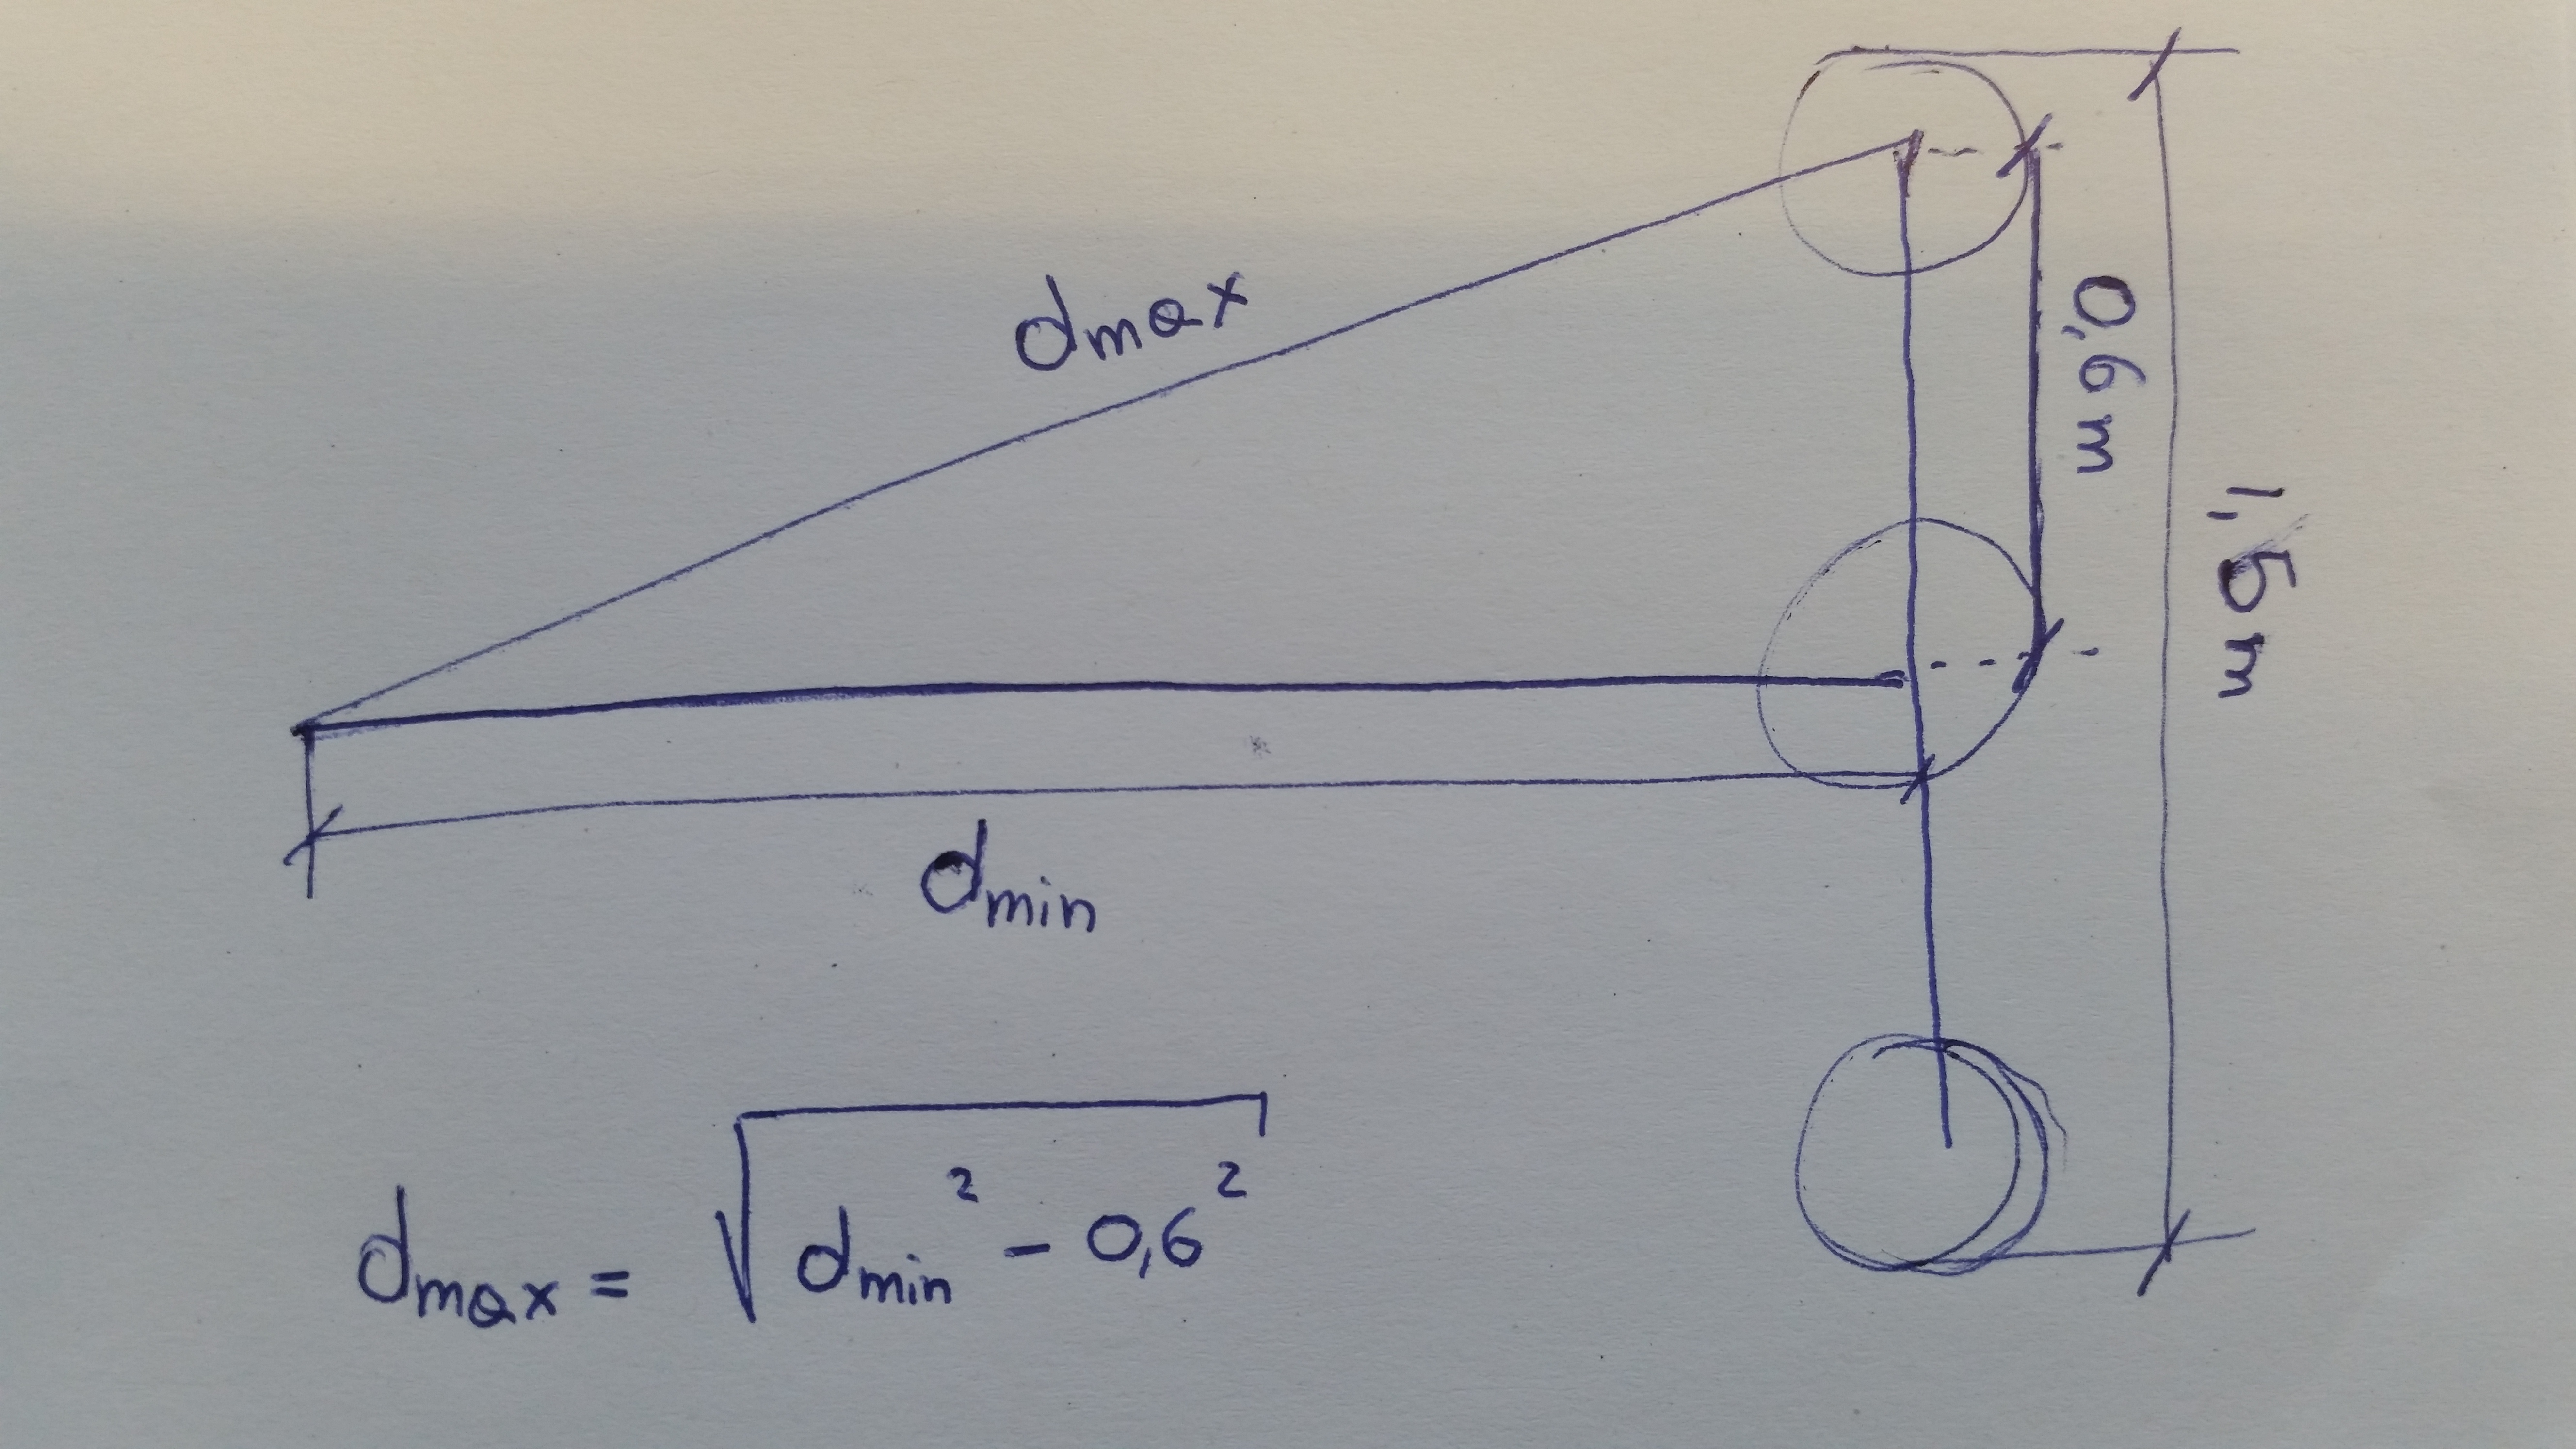
\includegraphics[width=1\textwidth]{../../fig/Skizze_Berechnung_2.jpg}
		\caption{Schrägen Wurf von Oben}
		\label{fig:Berechnungen von die Geschwindigkeit}
	\end{subfigure}
	\caption{Berechnung schräger Wurf}
	\label{Berechnungen}
\end{figure}

\begin{gather}
	v=\frac{\sqrt{g} \cdot d}{\sqrt{2} \cdot cos(\alpha) \cdot \sqrt{d \cdot tan(\alpha)+(h_0-h_1)}}\\
	\omega=\frac{v_{tan}}{r}\\
	f=\frac{\omega}{2\pi}\\
	rpm=60 \cdot f
\end{gather}

Unsere Berechnungen ergaben eine minimale Abwurfgeschwindigkeit von 4.18 m/s und eine Drehzahl von 532 U/min bei der kleinsten Wurfdistanz ($d_{min}$), 
Für die grösstmögliche Wurfdistanz ($d_{max}$) ergibt dies  eine Geschwindigkeit von 4.29 m/s und eine Drehzahl von 546 U/min. 
Die Abweichung liegt bei rund 2.5\%, und wird mit der Steuerung des Motors angepasst.
Der Maximale Winkel zwischen der Mitte des Spielfeldes und der äussersten Position des Kübels $\alpha_{max}$ beträgt 19°. \\
Bei diesen Berechnungen sind Faktoren wie Reibung etc. nicht berücksichtigt. Aus diesem Grund sind die Resultate als Mindestanforderungen zu betrachten.\\ \\
Um eine Schätzung der Drehmoment haben wir Berechnet, wie wenn der Ball ein Masse von 1 Kg hätte und der Drehrad als Hebelarm wäre. Mit diese Annahme wurde die Berechnung mit die Formeln\\
\begin{gather}
	M_{Drehmoment}=F*r
\end{gather}\\
und haben ein Drehmoment von 1.01 Nm bekommen. Auch in diesem Fall nehmen wir das als Mindestanforderung an.\\
Da wir eine Riemenscheibe benutzen werden, haben wir der Drehmoment der Motor mit einem Übersetzungsverhältnis von i=4 berechnet.\\
\begin{gather}
	M_{Antrieb}=\frac{M_{Abtrieb}}{i}
\end{gather}\\
Um auf die sichere Seite zu bleiben nehmen wir an das wir einem Drehmoment von 2 Nm am Rad ergibt es 0.5 Nm am Motor.\\ \\
Für die Berechnungen vom Schrittmotor der für die Drehung zuständig ist, haben wir die Maschine auf 2 Teile reduziert: Platte und Aufbau.
Die Platte ist ein Zylinder mit $r=0.25$m und $h=0.005$m, da die Durchschnittliche Dichte der Holz ist $750 Kg/m^2$, ergibt sich eine Masse von ca. 0.75 Kg.
Der Aufbau ist ein Quader mit $l=0.5$m, $b=0.01$m und wir schätzen eine Masse von 4 Kg.\\
Mit diese Daten wurde möglich der Trägheitsmoment berechnen.\\
\begin{gather}
	I_{Platte}=\frac{1}{2}*m*r^2 \\
	I_{Aufbau}=\frac{1}{12}*m*(l^2+b^2)
\end{gather}\\
Das Gesamte Trägheitsmoment ist denn $I=0.18 Kg*m^2$.\\
Die Maschine, wenn es in der Mitte der Spielfeld situiert wird, muss sich maximal um 19° Drehen in eine oder die andere Richtung. Wenn wir für die Umdrehung 1 Sekunde feststellen, können wir die Winkelbeschleunigung berechnen. \\
\begin{gather}
	\theta(t)=\theta_0+\omega_0*t+\frac{1}{2}*\alpha*t^2
\end{gather}\\
Wir erhalten so einen Winkelbeschleunigung $\alpha$ von 0.66$\frac{rad}{s^2}$.\\
Mit der Trägheitsmoment und der Winkelbeschleunigung wurde uns möglich der Drehmoment zu Berechnen.
Mit die Formeln $M=\alpha*I$ erhalten wir ein Drehmoment von 0.12 Nm.\\ \\
Für der Motor der für der Ballvorschub zuständig ist, haben wir so berechnet, wie wenn er alle 5 Bälle vertikal aufheben sollte.\\
Die 5 Bälle haben eine Masse von $60*5=300$ g. Diese 300g machen eine Kraft $F_g=0.3*9.81\approx3 N$. Wenn diese Kraft wie ein Hebelarm Betrachtet wird, können wir als Abstand etwas grösser als der Radius der Bälle ($r=3.7cm$) Benutzen. Nach unseres Aufbau ist dieses Abstand klein, und haben 5 cm für die Berechnung benutzt. Der Drehmoment auf der Motor wird denn, aus $M=F*r$, 0.15 Nm.\\
\newpage

\subsubsection{Sichtfeld der Kamera}
\label{subsub:sichtfeld-der-kamera}
Damit sichergestellt werden kann dass die Kamera das gesamte Spielfeld fotografieren kann, wird in diesem Abschnitt das Sichtfeld der Kamera berechnet. Auf der Website von \citeauthor{raspberry-pi-camera} \citeyear{raspberry-pi-camera} wurden diverse Tests mit dem Raspberry Pi Camera Modul (siehe Abschnitt \ref{subsub:kamera}) durchgeführt. Diese haben ergeben dass die Kamera ein horizontales Sichtfeld von $53^\circ$ und ein vertikales Sichtfeld von $40^\circ$ hat. Wie man der Abbildung \ref{fig:berechnung_sichtfeld} entnehmen kann ergibt das bei einer Distanz von zwei Meter eine Aufnahmefläche von 2×1.3 Meter.

\begin{figure}[h!]
\centering
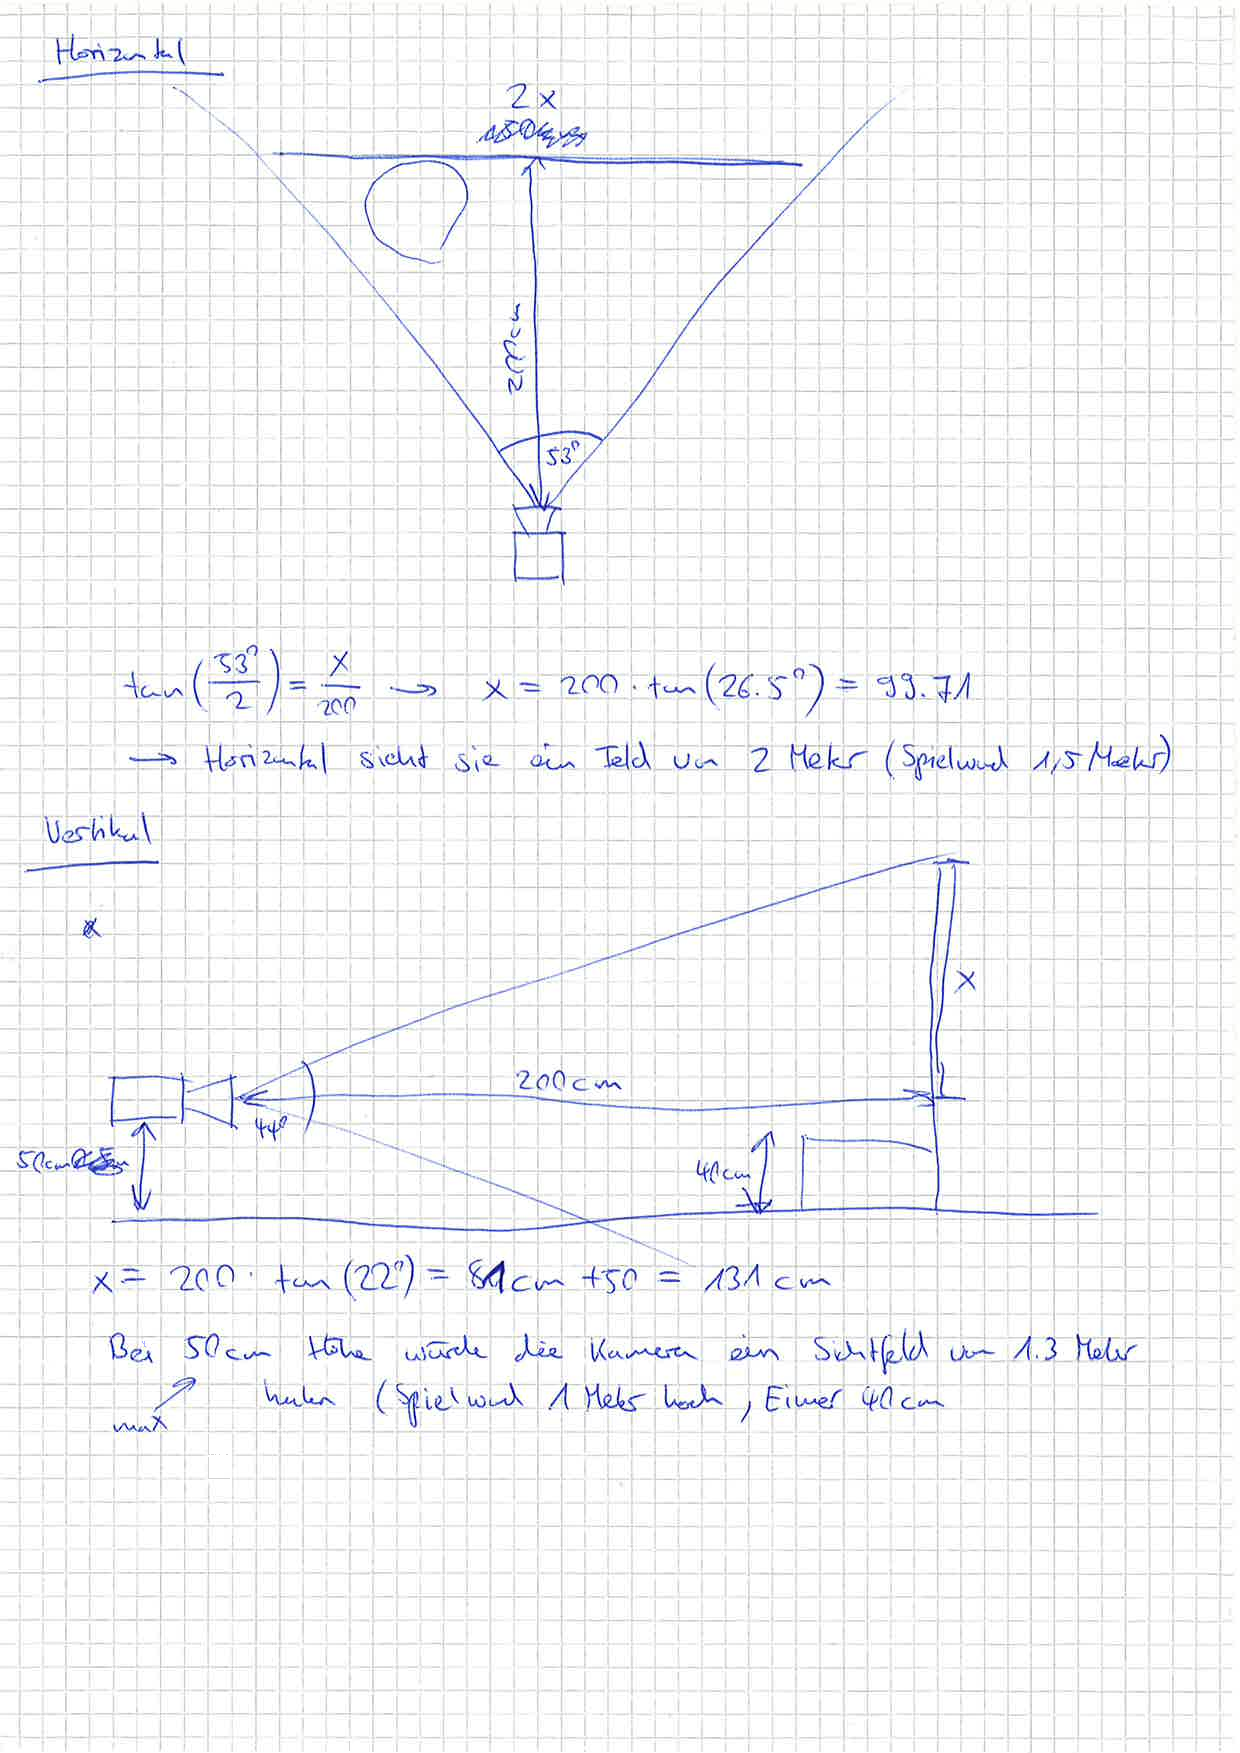
\includegraphics[width=0.6\linewidth]{../../fig/berechnung_sichtfeld.pdf}
\caption{Berechnung des Sichtfeldes der Kamera}
\label{fig:berechnung_sichtfeld}
\end{figure}

\subsubsection{Weitere Berechnungen}
Detailliertere Berechnungen sind im Anhang zu finden (siehe \ref{anhang-Berechnungen})